
 \documentclass[12pt]{article}
\usepackage{graphicx}
\usepackage{booktabs}
 \usepackage{makecell}
 \usepackage{float}
 \newcommand{\diff}{\,\mathrm{d}}
\usepackage[margin=1in]{geometry}
\usepackage{fancyhdr}
\pagestyle{fancy}
\usepackage{extarrows}
\usepackage{breqn}

\newcommand{\N}{\mathbb{N}}
\newcommand{\Z}{\mathbb{Z}}
\newcommand{\trans}{^{\mathrm T}}
\usepackage{amssymb}
\usepackage[table]{xcolor}
\usepackage{bm}
\usepackage{array}
\usepackage{mathtools}
\usepackage[english]{babel}
\usepackage{natbib}
\usepackage{url}
\usepackage[utf8x]{inputenc}
\usepackage{amsmath}
\usepackage{graphicx}
\graphicspath{{images/}}
\usepackage{parskip}
\usepackage{fancyhdr}
\usepackage{vmargin}
\usepackage[font={bf, footnotesize}, textfont=md]{caption}
\usepackage{amsmath,amsthm,amssymb}


\newenvironment{theorem}[2][Theorem]{\begin{trivlist}
\item[\hskip \labelsep {\bfseries #1}\hskip \labelsep {\bfseries #2.}]}{\end{trivlist}}
\newenvironment{lemma}[2][Lemma]{\begin{trivlist}
\item[\hskip \labelsep {\bfseries #1}\hskip \labelsep {\bfseries #2.}]}{\end{trivlist}}
\newenvironment{exercise}[2][Exercise]{\begin{trivlist}
\item[\hskip \labelsep {\bfseries #1}\hskip \labelsep {\bfseries #2.}]}{\end{trivlist}}
\newenvironment{reflection}[2][Reflection]{\begin{trivlist}
\item[\hskip \labelsep {\bfseries #1}\hskip \labelsep {\bfseries #2.}]}{\end{trivlist}}
\newenvironment{proposition}[2][Proposition]{\begin{trivlist}
\item[\hskip \labelsep {\bfseries #1}\hskip \labelsep {\bfseries #2.}]}{\end{trivlist}}
\newenvironment{corollary}[2][Corollary]{\begin{trivlist}
\item[\hskip \labelsep {\bfseries #1}\hskip \labelsep {\bfseries #2.}]}{\end{trivlist}}
\DeclareMathOperator{\tr}{tr}
\DeclareMathOperator{\rank}{rank}
\DeclareMathOperator{\Span}{span}
\DeclareMathOperator{\row}{row}
\DeclareMathOperator{\col}{col}
\DeclareMathOperator{\range}{range}
\DeclarePairedDelimiterX{\inp}[2]{\langle}{\rangle}{#1, #2}
\DeclareMathOperator{\Proj}{Proj}
\DeclareMathOperator{\trace}{trace}
\newcommand{\Her}{^{\mathrm H}}
\DeclareMathOperator{\diag}{diag}
\makeatletter 
    \newcommand\fcaption{\def\@captype{table}\caption}
\makeatother
\setmarginsrb{3 cm}{2.5 cm}{3 cm}{2.5 cm}{1 cm}{1.5 cm}{1 cm}{1.5 cm}
\setlength\parindent{1em}

\title{Short Report: Large Amplitude Pendulum}                             % Title
\author{Chen Ang}                               % Author
\date{\today}                                           % Date

\makeatletter
\let\thetitle\@title
\let\theauthor\@author
\let\thedate\@date
\makeatother

\pagestyle{fancy}
\fancyhf{}
\rhead{\theauthor}
\lhead{\thetitle}
\cfoot{\thepage}

\begin{document}

%%%%%%%%%%%%%%%%%%%%%%%%%%%%%%%%%%%%%%%%%%%%%%%%%%%%%%%%%%%%%%%%%%%%%%%%%%%%%%%%%%%%%%%%%

\begin{titlepage}
    \centering
    \vspace*{0.5 cm}
    
\includegraphics[scale = 0.75,width=6cm]{CUHK}\\[1.0 cm]   % University Logo
    \textsc{\large The Chinese University of Hong Kong, Shenzhen}\\[2.0 cm]   % University Name
    \textsc{\Large PHY 1002}\\[0.5 cm]               % Course Code
    \textsc{\large Physics Laboratory}\\[0.5 cm]               % Course Name
    \rule{\linewidth}{0.2 mm} \\[0.4 cm]
    { \huge \bfseries \thetitle}\\
    \rule{\linewidth}{0.2 mm} \\[1.5 cm]
    
    \begin{minipage}{0.4\textwidth}
        \begin{flushleft} \large
            \emph{Author:}\\
            \theauthor
            \\
            \emph{Group Number:} \\
            Group 1
            \end{flushleft}
            \end{minipage}~
            \begin{minipage}{0.4\textwidth}
            \begin{flushright} \large
            \emph{Student Number:} \\
            118010009                                   % Your Student Number
            \\
            \emph{Experiment Date:}\\
            September 27, 2019
        \end{flushright}
    \end{minipage}\\[2 cm]
    
    {\large \thedate}\\[2 cm]
 
    \vfill
    
\end{titlepage}

%%%%%%%%%%%%%%%%%%%%%%%%%%%%%%%%%%%%%%%%%%%%%%%%%%%%%%%%%%%%%%%%%%%%%%%%%%%%%%%%%%%%%%%%%
%%%%%%%%%%%%%%%%%%%%%%%%%%%%%%%%%%%%%%%%%%%%%%%%%%%%%%%%%%%%%%%%%%%%%%%%%%%%%%%%%%%%%%%%%

\tableofcontents
\pagebreak


%%%%%%%%%%%%%%%%%%%%%%%%%%%%%%%%%%%%%%%%%%%%%%%%%%%%%%%%%%%%%%%%%%%%%%%%%%%%%%%%%%%%%%%%%

\rmfamily

\section{Introduction}

This experiment explored the relationship between the wavelength, speed, and frequency of sound waves in a tube. Part 1 of the experiment investigated sound waves in a closed tube (closed on one end.) Experimental value of the speed of the sound waves was calculated and compared with the actual value as verification of the theory. Part 2 of the experiment investigated sound waves in an open tube. The wavelength of the sound waves, as well as the effective length of the tube were calculated. The ratio of the open-tube frequency and the close-tube frequency of the first harmonic was found.

\section{Setup}
Put an adjustable foot on each end of the tube, about 2 cm near the end. Tighten (but do not over-tighten) the screws that hold the feet in place. After this, place the Mini Speaker at one end of the tube with the Mini Speaker housing inside the tube. Insert the piston into the other end of the tube. Connect the Mini Speaker to the Universal Interface.
\begin{figure}[htb]
	\center{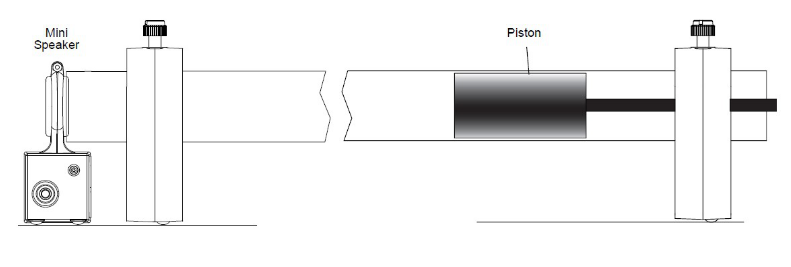
\includegraphics[width=\textwidth]
	{1.png}}
	\caption{\label{1} Air Column Setup}
\end{figure}


\section{Experiment (Part 1)}
In part 1 of the experiment, we explored the relationship between the wavelength, speed, and frequency of sound waves in a closed tube.
\subsection{Theory}
In a closed tube, the resonating air column will always have a node fixed on the closed end and an anti-node on the open end. Therefore, the resonances happen when the wavelength,  $\lambda,$ and the length of the tube, $L,$  satisfy $$L= \frac {n\lambda}4,n=1,3,5,\cdots$$

At the fundamental harmonic of resonance ($n=1$),
$$\lambda=4L$$
Rewriting the equation with the fact that
$$
v = \lambda f
$$
we have
\begin{equation}
L = \frac v4 f^{-1} = \frac v4 T \label{eq:1}
\end{equation}
where $v$ is the wave speed, $f$ the frequency of the wave, $T$ the period.

With the speed of sound fixed in the air, the length of the column $L$ is inversely proportional to the fundamental frequency $f$, with coefficient $v/4.$ Equivalently, it is proportional to the period $T$, with coefficient $v/4.$

\subsection{Procedure}
The piston was used to vary the length of the resonating column, starting from 110 cm to 40 cm at last, with a step of 10 cm. For each length of the column, the signal generator produced a sweep type sound wave of frequency from $f_0$ to $f_t$ in a span of time $t.$ The step of the frequency was $1$ Hz. The sound intensity graph on PASCO Capture was used to locate the resonating frequency (when sound intensity was highest) of each length.


\subsection{Raw Data}

With the intensity graphs provided by PASCO Capture (See Figure 8 in Appendix), we should have been able to locate the fundamental frequencies to the nearest 1 Hz. Nevertheless, locating the exactly position of the resonance proved to be rather challenging. Adding to the considerable noise in the experiment environment polluting the data, we were unable to reduce the uncertainty any further than $\delta_f = 1$ Hz. Consequently, the propagation error in $T$ was
$$
\delta_{T}=|\frac d {df}f^{-1}||\delta_f| = f^{-2} \text{ Hz}
$$
And the length of each air column was measured with an uncertainty of $\delta_L = 1$ cm.

The identified fundamental frequency and the corresponding period for each column length can be found in Table \ref{tab1}.

\begin{table}
	\centering
\begin{tabular}{|c|c|c|}
	\hline 
	$L$ (cm) & $f$ (Hz) & $T$ (ms) \\ 
	\hline 
	110 $\pm 1$ & 78 $\pm 1$ & 12.821 $\pm 0.164$ \\ 
	\hline 
	100 $\pm 1$ & 85 $\pm 1$ & 11.765 $\pm 0.138$ \\ 
	\hline 
	90 $\pm 1$ & 95 $\pm 1$ &  10.526 $\pm 0.111$\\ 
	\hline 
	80 $\pm 1$ & 106 $\pm 1$ & 9.434 $\pm 0.089$ \\ 
	\hline 
	70 $\pm 1$ & 121 $\pm 1$ & 8.264 $\pm 0.068$\\ 
	\hline 
	60 $\pm 1$ & 138 $\pm 1$ & 7.246 $\pm 0.053$ \\ 
	\hline 
	50 $\pm 1$ & 166 $\pm 1$ & 6.024 $\pm 0.036$ \\ 
	\hline 
	40 $\pm 1$ & 209 $\pm 1$ & 4.785 $\pm 0.023$ \\ 
	\hline
\end{tabular}
\caption{Raw Data of the Closed Tube}
\label{tab1}
\end{table}




\subsection{Calculating the Speed of Sound}
Plotting $T$ vs. $L$ on a graph, we obtained the fitted linear equation
$$
L = 87.5T - 0.0251
$$
with the uncertainty in the slope being $0.73,$ the intercept, $0.0067.$
\begin{figure}[!htb]
	\center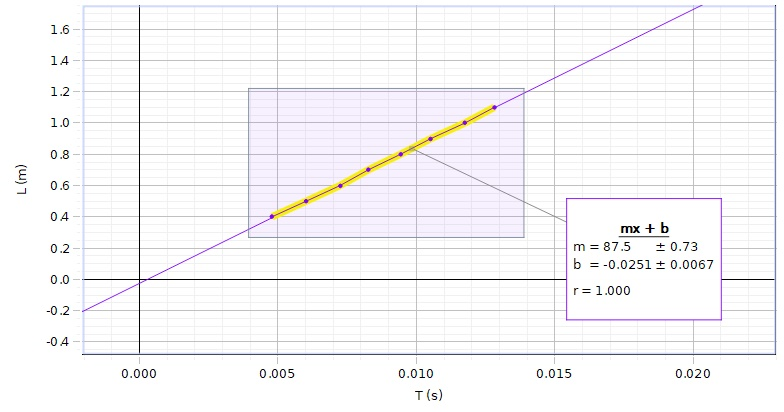
\includegraphics[width=0.6\textwidth]{lin}
	\caption{Linear Curve Fitting of $T$ vs. $L$}
\end{figure}


Using equation (\ref{eq:1}), we can now calculate the speed of sound by
$$
\begin{aligned}
v &= 87.5\times4\ \text{m/s}\\
&=350.00\pm{2.92}\ \text{m/s}
\end{aligned}
$$
which only differs from the actual value (340 m/s) by
$$
\frac{350-340}{340}=2.84\%
$$
\subsection{End Effect}
Curiously, the $y$ intercept of the fitting curve of $T$ vs. $L$ turned out to be negative ($-$2.51 cm), instead of zero predicted by equation (1). This was probably due to a known phenomenon named the \textbf{end effect}. Instead of forming exactly at the open end of the tube, the anti-node of the sound wave actually formed past the open end. This means that the effective length of the tube was constantly longer than measured, which causes a downward shift of the curve. The amount of this shift can be obtained empirically by the following formula
$$
\Delta L = 0.3\cdot D
$$
where $D$ is the diameter of the tube.

Using the meter ruler, we measured the diameter of the tube to be $3.8\pm 0.1$ cm. According to the formula above, the amount of the end effect would be
$$
0.3\times 3.8\text{ cm} = 1.14 \text{ cm}
$$
which, sadly, does not agree with our $2.51$-cm shift previously. Nevertheless, this is still reasonable as the formula is an empirical one, and thus may not be accurate enough to fully describe the phenomenon.
\subsection{Further Investigations}
We further investigated the relationship between the neighboring resonance modes, with the driving frequency fixed at $f= 230$ Hz. At column length $L_1= 112 \pm 1$ cm, a first resonance was identified. We then slowly decreased the length of the air column, until at $L_2=37\pm 1$ cm, another resonance was found.

Note that the distance between two resonant locations was
$$
d = L_1 - L_2 = 75\pm1.4\text{ cm}
$$
which should be a half of the wavelength. This is because at a fixed frequency, two neighboring resonant modes were formed at neighboring nodes, which were exactly $\lambda/2$ apart.
\begin{figure}[!htb]
	\center{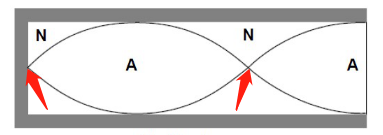
\includegraphics[width=0.6\textwidth]{f}}
	\caption{Two Neighboring Resonant Locations (Nodes)}
\end{figure}
This implies $\lambda=2d.$

Again, using the formula $v = \lambda f,$ we can find the speed of sound by
$$
\begin{aligned}
v&= 2\times75 \text{ cm}\times230\text{ Hz}\\
&= 345\pm6.51 \text{ m/s}
\end{aligned}
$$
which is only 1.43\% away from our previous value 350 m/s


\section{Experiment (Part 2)}
In Part 2 of the experiment, we explored the relationship between the wavelength, speed, and frequency of sound waves in an open tube.
\subsection{Theory}
In an open tube of length $L$, resonances happen when the wavelength $\lambda$ satisfies
$$
L = \frac{n\lambda}2, n = 1,2,3,\cdots
$$
Rewriting with $v = \lambda f$, we have
\begin{equation}
f_n = \frac{nv}{2L}, n = 1,2,3,\cdots
\end{equation}
where $v$ is the speed of sound, and $f_n$ is the $n$-th resonant frequency.
\subsection{Procedure}
The piston was removed from the air column so that two ends are open. The rest of the setup was identical to Part 1.

Starting from 50 Hz, A 1 Hz/s sweeping signal was again generated. Sound intensity graphs from the PASCO Capture were used to locate the frequencies of the first, second, and the third harmonic.

After finding the third harmonic, we kept the length of the tube constant and sealed one end of the tube with the piston. We decreased the driving frequency until the fundamental frequency of the closed tube was found. The ratio of the open-tube and close-tube fundamental frequencies were calculated.

\subsection{Raw Data}
Resonant frequencies were obtained from the intensity graphs provided by PASCO Capture (See Figure 9 in Appendix). The uncertainty remained to be $\delta_f$ = 1 Hz.
\begin{table}[h]
	\centering
	\begin{tabular}{l|lll}
		\hline
		\multicolumn{1}{c|}{Resonant Frequencies (Hz)} & $f_1$ & $f_2$ & $f_3$ \\ \hline
		Open & 138$\ \pm 1$ & 276$\ \pm 1$ & 407$\ \pm 1$ \\
		Closed & 71$\ \ \pm 1$ &  &  \\ \hline
	\end{tabular}
\caption{Resonant Frequencies of Open and Closed Tubes of Full Length}
\end{table}

\subsection{Discussions}
\begin{itemize}
	\item {\textbf{Open-Closed-Tube Ratio of $f_0$}}
	
		It was noticed that the fundamental frequency $f_0$ of the open tube was higher than that of the closed tube. In fact, the ratio turned out to be
		$$\begin{aligned}
		R&=\frac{f_o}{f_c}\\
		&=\frac{138\text{ Hz}}{71\text{ Hz}}\\
		&=1.944...\approx2
		\end{aligned}$$
		where the uncertainty was calculated via
		$$\begin{aligned}
		\delta_R &= \sqrt{
		\left(\frac{\partial R}{\partial f_o}\right)^2\delta^2_{f_o}+
			\left(\frac{\partial R}{\partial f_c}\right)^2\delta^2_{f_c}
	}\\
&= \sqrt{
\left(\frac{\delta_{f_0}}{f_c}\right)^2+
\left(f_0\frac{\delta_{f_c}}{f_c^2}\right)^2
}
\end{aligned}
$$
		This agreed with our previous theory. Acoording to equation (1), the fundamental frequency of a closed tube is
		$$
		f_{c}=\frac v{4L}
		$$
		Equation (2) evaluated at $n = 1$ yields
		$$
		f_{o}=\frac v{2L}
		$$
		Therefore,
		$$\begin{aligned}
		\frac{f_{o}}{f_{c}}&=\frac v{2L}\frac {4L}{v}=2
		\end{aligned}
		$$
This relation also holds for any number $n$ other than 1, according to the equations.
\newline
	\item {\textbf{$f_2$ Closed = $f_1$ Open}}
	
	When the driving frequency was returned to the fundamental of the open tube, and the tube was closed, a resonance was curiously present. This resonance, however, was too predicted by equation (1) and (2). Namely, since $$
	f_1 \text{ Open} = 2\cdot f_1 \text{ Closed}
	$$
	we have
	$$
	f_2 \text{ Closed} = f_1 \text{ Open}
	$$
	The resonance was the \emph{second} harmonic of the closed tube.
\newline
	\item {\textbf{End Effect}}
		
		Using equation (2) with $n=2,$ we calculated the effective length of the tube via
		$$
		L = \frac v {f_2}
		$$
		Here, we used the speed of sound found in Section 3.4
		$$
		v = 350.00\pm2.92\text{ m/s}
		$$
		Again, the uncertainty of the effective length was primarily due to the propagation, which was determined by
		$$
		\delta_{L}=\sqrt{
			\left(\frac{\delta_{v}}{f_2}\right)^2+
			\left(v\frac{\delta_{f_2}}{f_2^2}\right)^2
		}=1.15\text{ cm}
		$$
		Hence
		$$
		L = 126.81 \pm{1.15} \text{ cm}
		$$
		The measured length of the resonating column was
		$$
		D = 120.00 \pm 1.00\text{ cm}
		$$
		from which we calculated the amount of end effect
		$$
		\Delta{L} = L - D
		$$
		where the uncertainty was given by
		$$
		\delta_{\Delta L}=\sqrt{
	\delta_L^2+\delta_D^2
	} = 1.53\text{ cm}
		$$
		Therefore, the amount of end effect was
		$$
		\Delta L = 6.81 \pm 1.53\text{ cm}
		$$
		Again, unfortunately, this value did not agree with the empirical formula (from which we would have 1.14 cm $\times$ 2 = 2.28 cm.) However it was rather consistent with our previous $2.51$-cm end effect with one open end, as the amount of end effect was approximately doubled with two open ends.
\end{itemize}

\subsection{Further Investigations}
In a closed tube, the even harmonics cannot be formed. This is because the closed end of the tube will always be a node whereas the open end will always be an anti-node. With even harmonics, if the closed end forms a node, the open end will also form a node instead of an anti-node, whence impossible.

The relationship between the tube length $L$ and the wavelength $\lambda$ of the third harmonic of a closed tube is given by$
L = \frac34\lambda.
$
\newpage
\begin{figure}[!htb]
	\center{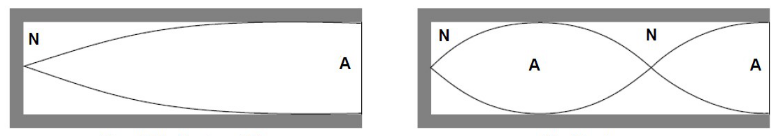
\includegraphics[width=0.8\textwidth]{hh}}
	\caption{First and Third Harmonics in a Closed Tube with Fixed Length}
\end{figure}
In Figure 4, the length of the tube is forced at constant while the frequency (wavelength) is allow to change. This is different from the case in Figure 3, Part 1, where the frequency (wavelength) was forced to stay constant, but the length of the tube could vary.
\appendix
\section{Raw Figures}
The following pages contain the sound intensity graphs taken from PASCO Graphic in the experiment. Figure 5 is of Part 1, Figure 6 Part 2.
\clearpage
\begin{sidewaysfigure}
	\centering
	\subfloat[110 cm]{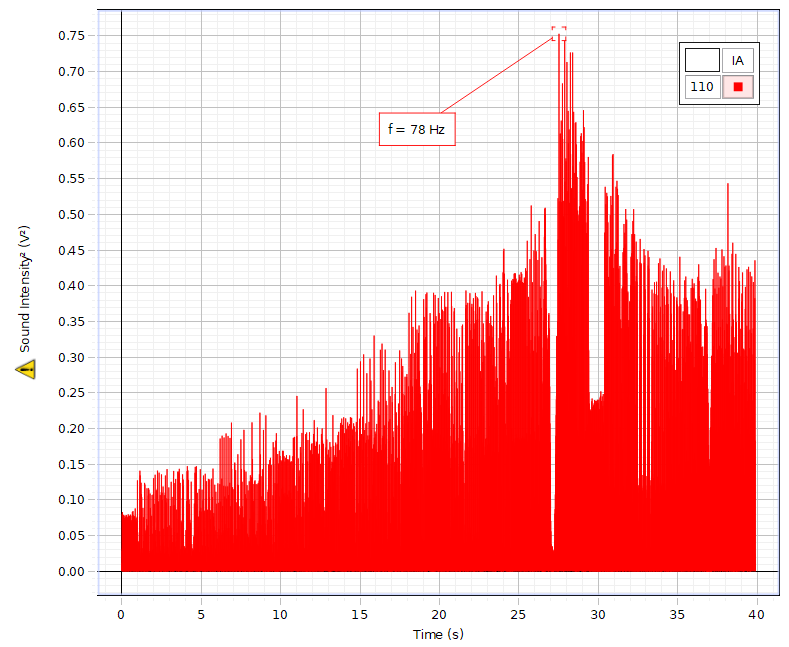
\includegraphics[width=0.4\textheight]{2}\label{fig:a}} \hspace{40pt}
	\subfloat[100 cm]{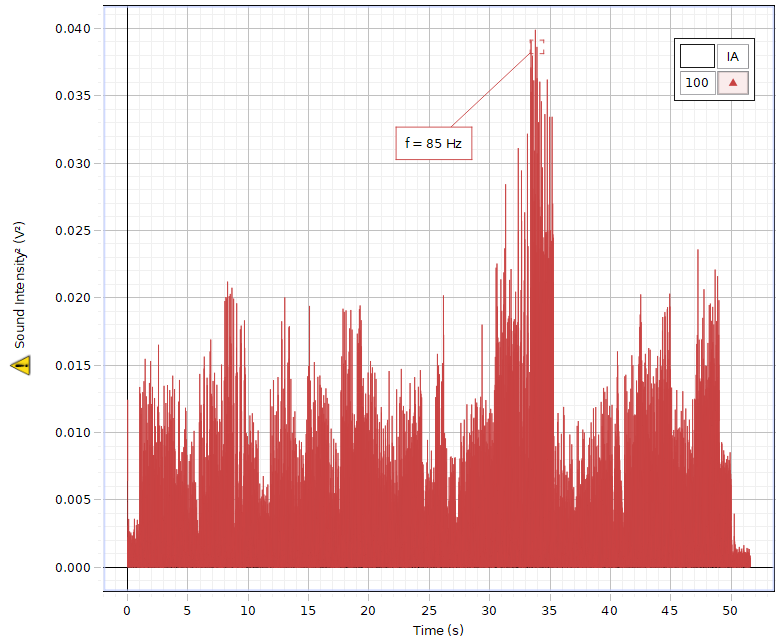
\includegraphics[width=0.4\textheight]{3}\label{fig:b}}\\
	\subfloat[90 cm]{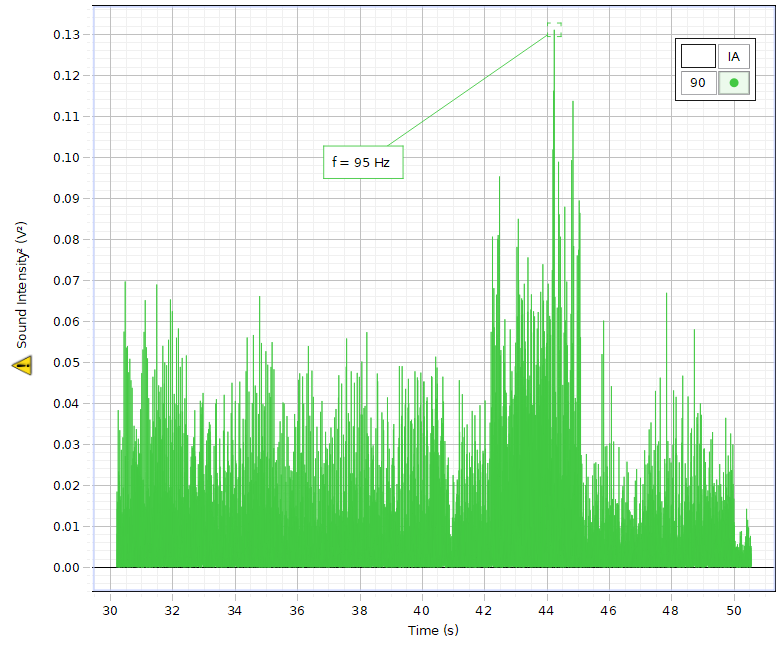
\includegraphics[width=0.4\textheight]{4}\label{fig:c}}\hspace{40pt}
	\subfloat[80 cm]{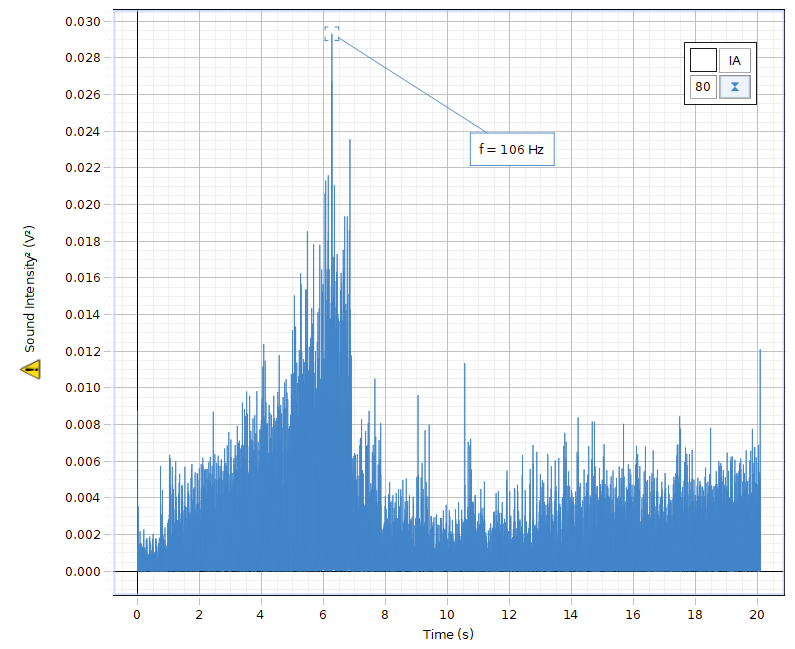
\includegraphics[width=0.4\textheight]{5}\label{fig:c}}
	\caption{Sound Intensity$^2$ During 1 Hz/s Sweeping Signals in Closed Air Columns of Varied Length\label{fig:test}}
\end{sidewaysfigure}
\begin{sidewaysfigure}\ContinuedFloat
	\centering
	\subfloat[70 cm]{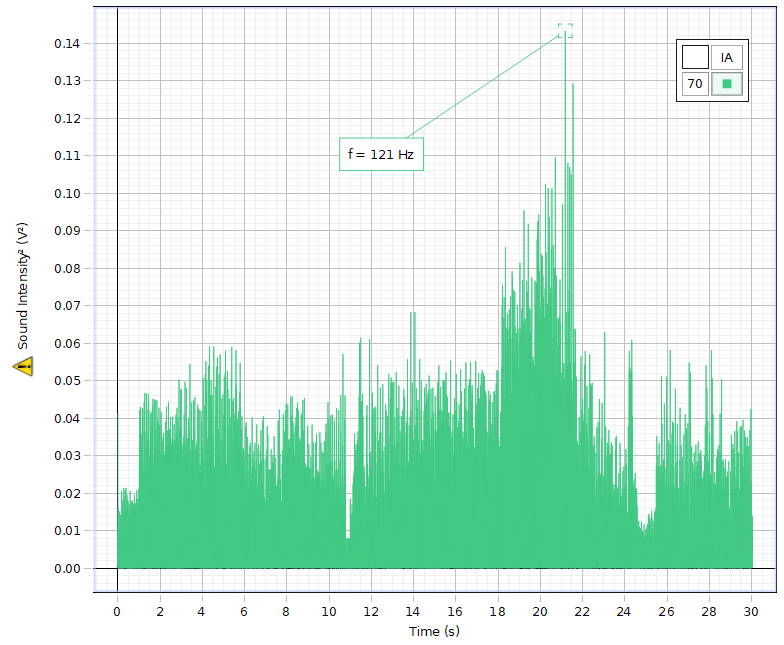
\includegraphics[width=0.4\textheight]{6}\label{fig:a}} \hspace{40pt}
	\subfloat[60 cm]{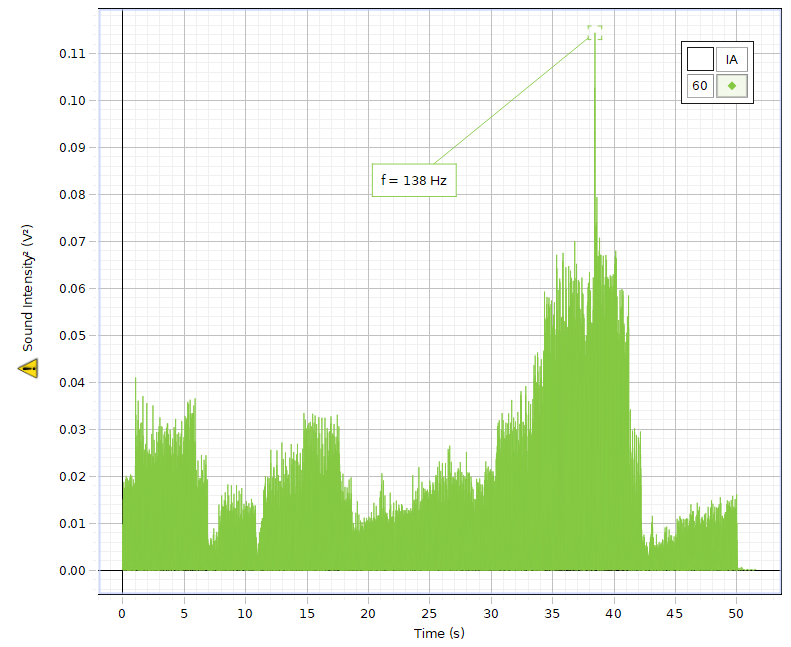
\includegraphics[width=0.4\textheight]{7}\label{fig:b}}\\
	\subfloat[50 cm]{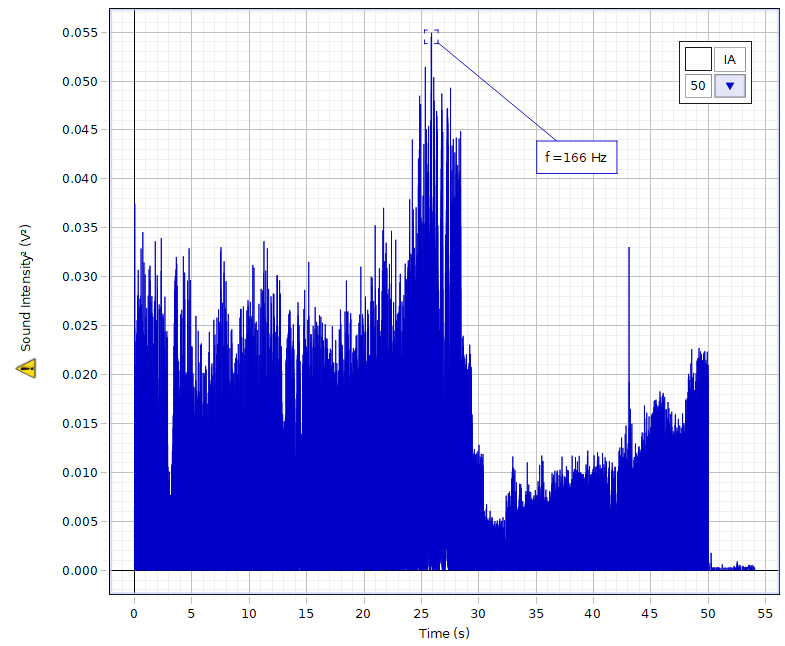
\includegraphics[width=0.4\textheight]{8}\label{fig:c}}\hspace{40pt}
	\subfloat[40 cm]{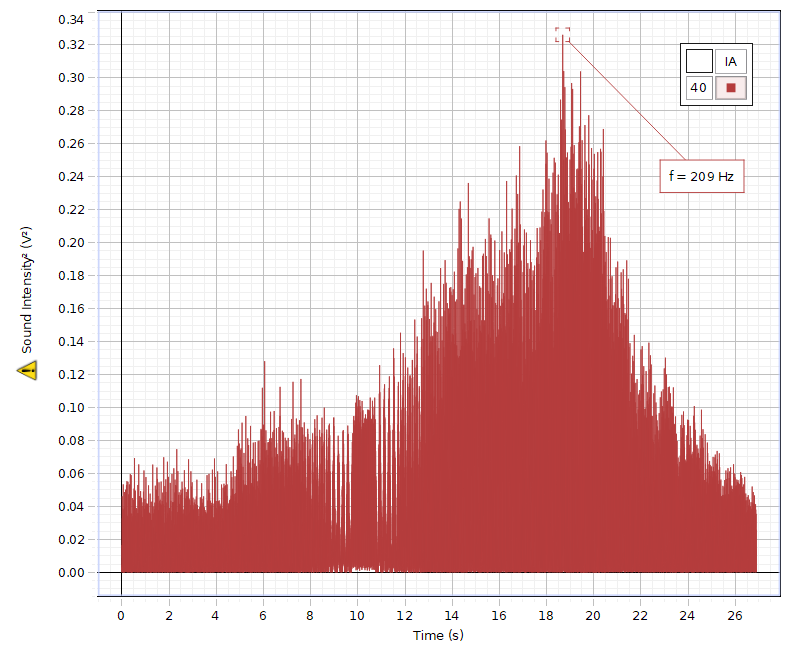
\includegraphics[width=0.4\textheight]{9}\label{fig:c}}
	\caption{Sound Intensity$^2$ During 1 Hz/s Sweeping Signals in Closed Air Columns of Varied Length (Continued)\label{fig:test}}
\end{sidewaysfigure}
\clearpage
\newpage

\begin{sidewaysfigure}[!htb]
	\centering
	\subfloat[First Harmonic (Open)]{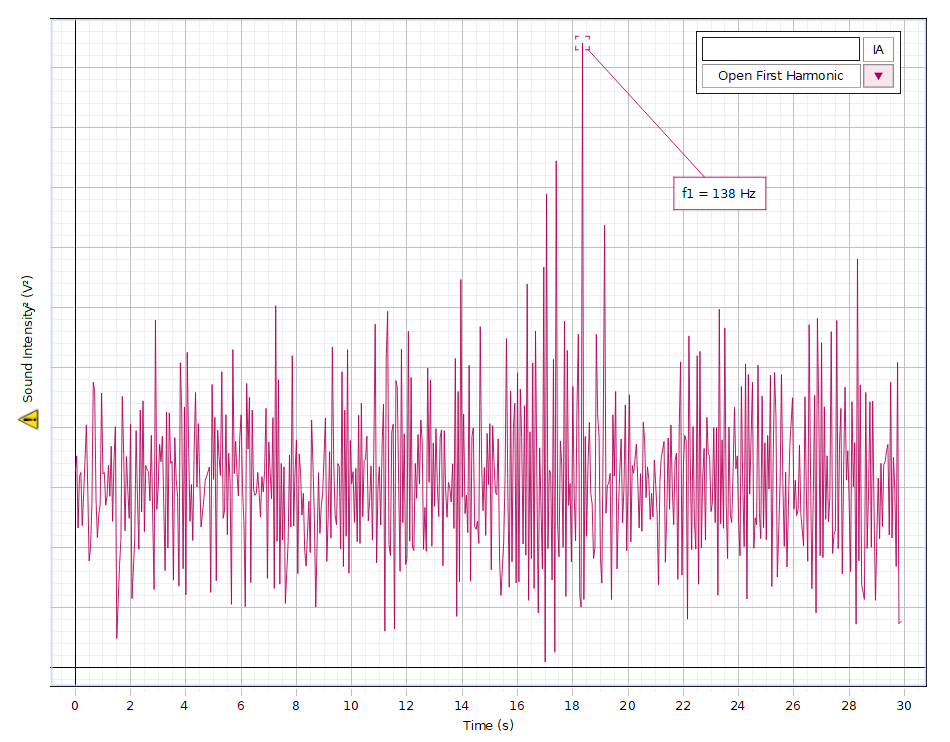
\includegraphics[width=0.4\textheight]{a}\label{fig:a}} \hspace{40pt}
	\subfloat[Second Harmonic (Open)]{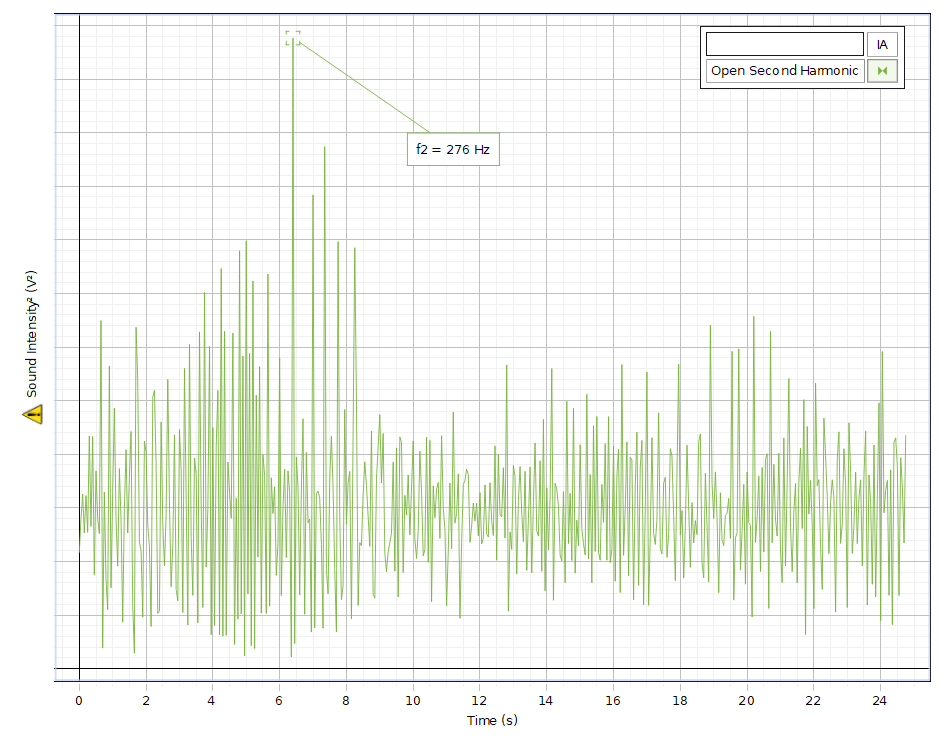
\includegraphics[width=0.4\textheight]{b}\label{fig:b}}\\
	\subfloat[Third Harmonic (Open)]{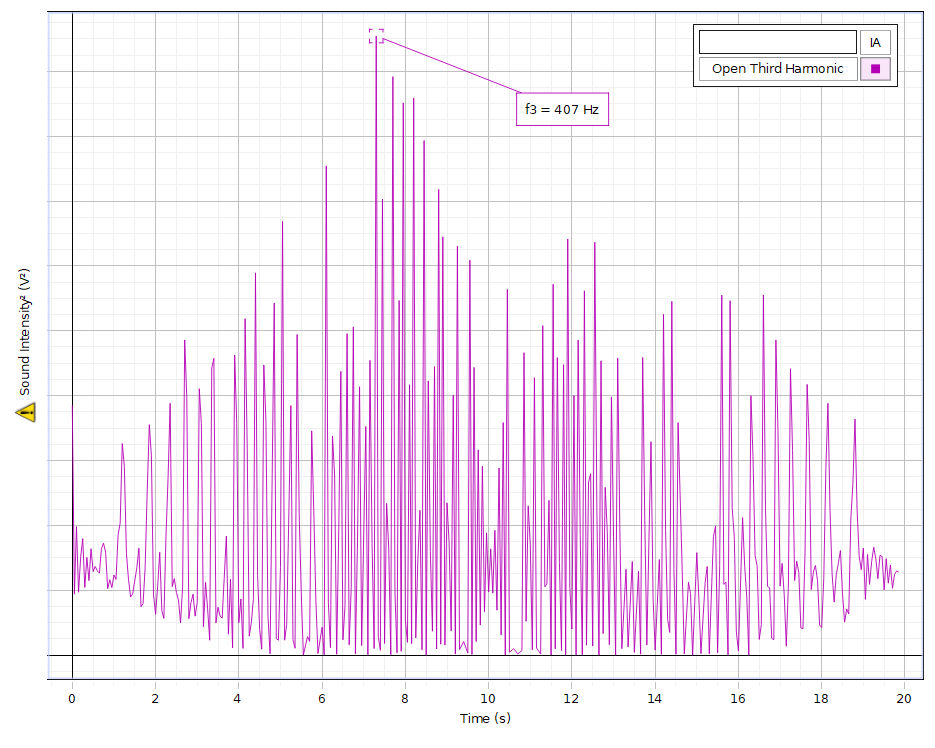
\includegraphics[width=0.4\textheight]{c}\label{fig:c}}\hspace{40pt}
	\subfloat[First Harmonic (Closed)]{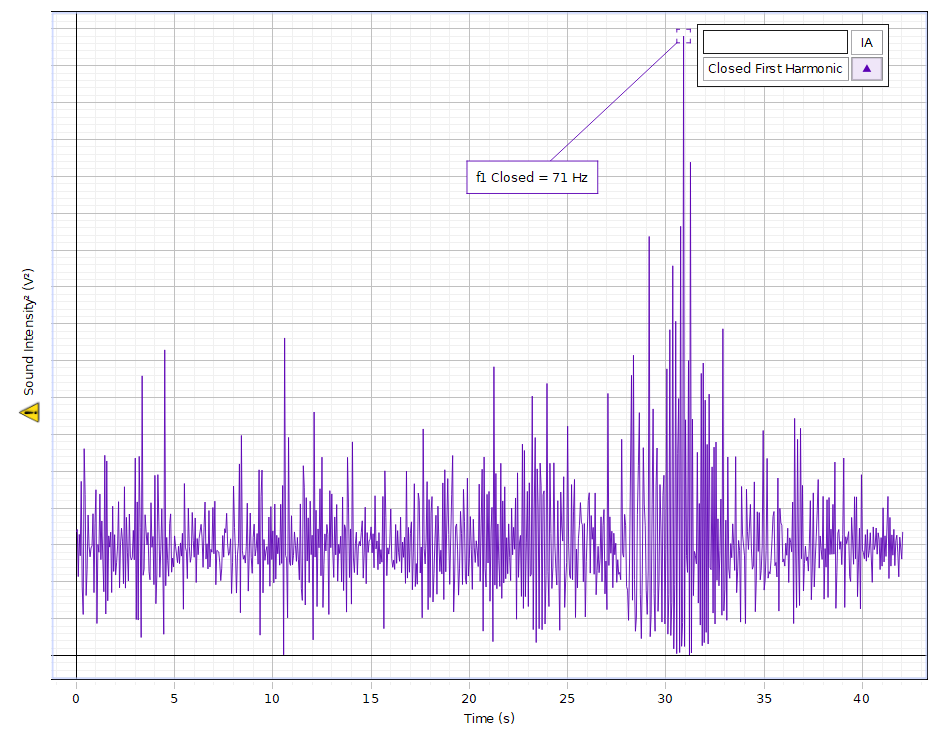
\includegraphics[width=0.4\textheight]{d}\label{fig:c}}
	\caption{Sound Intensity$^2$ During 1 Hz/s Sweeping Signals in Open and Closed Air Columns of Full Length\label{fig:test}}
\end{sidewaysfigure}
\clearpage
\end{document}